\documentclass[12pt, a4paper]{article}

% Text languages
\usepackage[english, UKenglish, USenglish, american, british]{babel}

% Accents
%usepackage[latin1]{inputenc}

% Maths
\usepackage{mathtools}
\usepackage{amsmath,amsthm,amssymb}

% Double rows
%\usepackage{multirow}

% Math-mode symbol & verbatim
%\def\W#1#2{$#1{#2}$ &\tt\string#1\string{#2\string}}
%\def\X#1{$#1$ &\tt\string#1}
%\def\Y#1{$\big#1$ &\tt\string#1}
%\def\Z#1{\tt\string#1}

% A non-floating table environment.
%\makeatletter
%\renewenvironment{table}%
%   {\vskip\intextsep\parskip\z@
%    \vbox\bgroup\centering\def\@captype{table}}%
%   {\egroup\vskip\intextsep}
%\makeatother

%\DeclarePairedDelimiter\abs{\lvert}{\rvert}%
%\DeclarePairedDelimiter\norm{\lVert}{\rVert}%

% Swap the definition of \abs* and \norm*, so that \abs
% and \norm resizes the size of the brackets, and the 
% starred version does not.
%\makeatletter
%\let\oldabs\abs
%\def\abs{\@ifstar{\oldabs}{\oldabs*}}
%
%\let\oldnorm\norm
%\def\norm{\@ifstar{\oldnorm}{\oldnorm*}}
%\makeatother

% C++
\usepackage{listings}
\usepackage{xcolor}
\lstset { %
	language = C++,
	backgroundcolor=\color{black!5}, % set backgroundcolor
    basicstyle=\footnotesize,% basic font setting
    tabsize=4, % tab space width
    showstringspaces=false, % don't mark spaces in strings
    %numbers=left, % display line numbers on the left
    commentstyle=\color{green}, % comment color
    keywordstyle=\color{blue}, % keyword color
    stringstyle=\color{red} % string color
}

% https://www.overleaf.com/learn/latex/Page_size_and_margins
\usepackage{geometry}
\topmargin = -23pt
\oddsidemargin = 13pt
\headheight = 12pt
\headsep = 25pt
\textheight = 674pt
\textwidth = 426pt
\marginparsep = 10pt
\marginparwidth = 50pt
\footskip = 30pt
\marginparpush = 5pt
\hoffset = 0pt
\voffset = 0pt
\paperwidth = 597pt
\paperheight = 845pt

% Hyperlinks
\usepackage{hyperref}

% Figure
\usepackage{graphicx}
\usepackage{caption}
\usepackage{subcaption}
\usepackage{etoc}
% Example
\newtheorem{exmp}{Example}[section]
% Algorithms
%\usepackage[]{algorithm2e}
%\usepackage{algorithm}% http://ctan.org/pkg/algorithm
%\usepackage{algpseudocode}% http://ctan.org/pkg/algorithmicx
\usepackage{algpseudocode}

\renewcommand{\thefootnote}{\arabic{footnote}} % 1, 2, 3... (la que hay por defecto)

%\usepackage{titlesec}
%\setcounter{secnumdepth}{5}

%\titleformat{\paragraph}
%{\normalfont\normalsize\bfseries}{\theparagraph}{1em}{}
%\titlespacing*{\paragraph}
%{0pt}{3.25ex plus 1ex minus .2ex}{1.5ex plus .2ex}

\usepackage{float}
%--------------------------------------------------------------------------
\title{PARALLELISM}
\author{Roger Vilaseca Darné and Xavier Martín Ballesteros\\
  \small UNIVERSITAT POLITÈCNICA DE CATALUNYA\\
}
\date{10th December 2018}

\begin{document}
% Images
\graphicspath{ {./images} }

%\maketitle

\begin{titlepage}
	\centering
%	{\scshape\LARGE UNIVERSITAT POLITÈCNICA DE CATALUNYA \par}
	\vspace{1cm}
	{\scshape\Large UNIVERSITAT POLITECNICA DE CATALUNYA\par}
	\vspace{1.5cm}
	{\huge\bfseries PARALLELISM\par}
	\vspace{2cm}
	{\Large\itshape \textbf{Lab 2: Brief tutorial on OpenMP programming model}\par}
	\vfill
	{\Large\itshape Roger Vilaseca Darne and Xavier Martin Ballesteros\break PAR4110\par}
	\vfill
%	
\includegraphics[width=0.25\textwidth]{./images/UPC.png}\par\vspace{1cm}
	%supervised by\par
	%Dr.~Mark \textsc{Brown}

	\vfill

% Bottom of the page
	{\large 20th March 2019, Q1}
\end{titlepage}

%\abstract{Esto es una plantilla simple para un articulo en \LaTeX.}

%	*********************** ÍNDEX *********************
\setcounter{secnumdepth}{5}

\newpage
  \tableofcontents
\newpage

% Referència a una equació \ref{eq:area}).
% Referència a una secció \ref{sec:nada}
% Referència a una cita \cite{Cd94}.

\section{Introduction}

Talk about the Mandelbrot Set and about what we are going to do in this 3 sessions, in order.

\section{Task decomposition analysis with \textit{Tareador}}

In this section, we had to analyse the two possible task granularities that could be exploited in the given program. To do it, we used the \textit{Tareador} tool, which was very useful to see graphically the created tasks and which dependences are between them.

\subsection{Point decomposition}

In this decomposition strategy, a task corresponds with the computation of a single point (row, col) of the Mandelbrot set. Thus, we will have $row \times col$ tasks.

In order to analyse the potential parallelism of this strategy, we modified the code in \textit{mandel-tar.c} to create several \textit{Tareador} tasks. As we are using a point decomposition strategy, the tasks are created inside the most inner loop of the function mandelbrot.  Figure \ref{code:mandeltarPoint} shows the fragment of the function that we modified.

\begin{figure}[H]
\begin{lstlisting}
for (row = 0; row < height; ++row) {
	for (col = 0; col < width; ++col) {
		tareador_start_task("point");
		
		...
		
		tareador_end_task("point");
	}
}
\end{lstlisting}
\caption{Modified fragment of the \textit{mandel-tar.c} code.}
\label{code:mandeltarPoint}
\end{figure}

Once we did this, we executed interactively mandeld-tar and mandel-tar using run-tareador.sh script. The first one is used for timing purposes and to check for the numerical validity of the output (-o option) whereas with the second one we can visualize the Mandelbrot set.

The script has defined inside the size of the image to compute (-w option). In this case, the value was 8 to generate a reasonable task graph in a reasonable execution time. Hence, as we said before, the number of tasks will be $8 \times 8 = 64$.

Figures \ref{fig:mandel-tar-point} and \ref{fig:mandeld-tar-point} below show the two task decomposition graphs (TDG) of the two possible executions. There are some nodes bigger than the others. This is because these nodes have executed more instructions than the rest. Therefore, these nodes represent pixels in white\footnote{The bigger the node, the more iterations it does in the do while fragment of the function. This make that the computed color is white.}.

\begin{figure}[H]
	\centering
	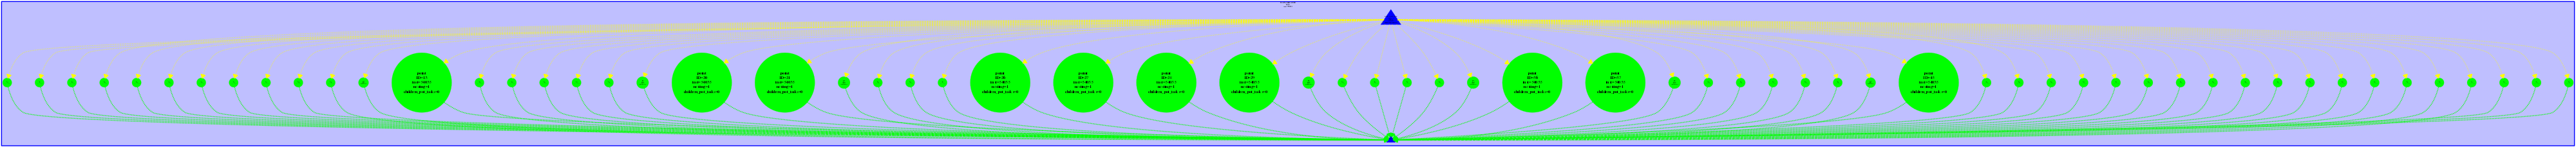
\includegraphics[scale=0.106]{./mandel-tar_point}
	\caption{Mandel-tar task decomposition graph using the point decomposition strategy.}
	\label{fig:mandel-tar-point}
\end{figure}

\begin{figure}[H]
	\centering
	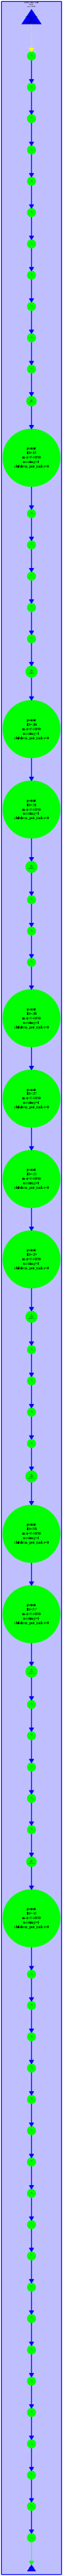
\includegraphics[scale=0.106]{./mandeld-tar_point}
	\caption{Mandeld-tar task decomposition graph using the point decomposition strategy.}
	\label{fig:mandeld-tar-point}
\end{figure}

This strategy will have more overhead of creation and termination of tasks than in the row strategy because it has to create more tasks. However, as a positive point the tasks are better distributed because if in a row there are many white areas, this work will not only be done by a single thread. Thus, it may end the execution earlier than in the row decomposition strategy.

\subsection{Row decomposition}

In this other strategy, a task corresponds with the computation of a whole row of the Mandelbrot set. This strategy only creates $row$ tasks.

In this case, the code is not the same as before. We changed the creation of the \textit{Tareador} tasks so that each time we enter a new row (second loop) a new task is created. The modified version of the code is shown below.

\begin{figure}[H]
\begin{lstlisting}
for (row = 0; row < height; ++row) {
	tareador_start_task("row");
	for (col = 0; col < width; ++col) {
		...
	}
	tareador_end_task("row");
}
\end{lstlisting}
\caption{Modified fragment of the \textit{mandel-tar.c} code.}
\label{code:mandeltarRow}
\end{figure}

Afterwards, we executed interactively mandel-tar and mandeld-tar again. We used the same size as before. Hence, the total number of tasks will be 8. The graphical results we got can be seen in figures \ref{fig:mandel-tar-row} and \ref{fig:mandeld-tar-row}.

\begin{figure}[H]
	\centering
	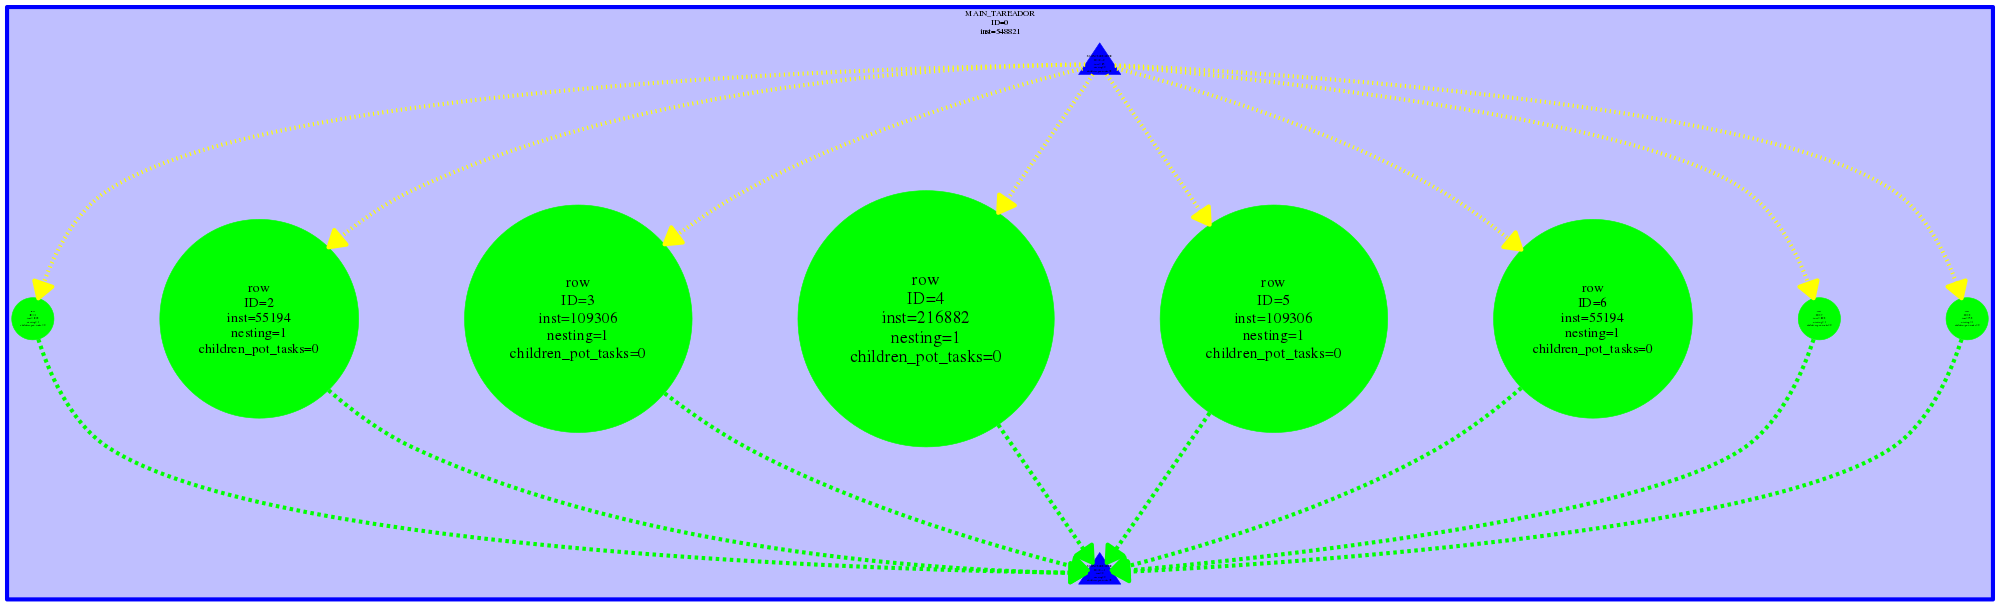
\includegraphics[scale=0.106]{./mandel-tar_row}
	\caption{Mandel-tar task decomposition graph using the row decomposition strategy.}
	\label{fig:mandel-tar-row}
\end{figure}

\begin{figure}[H]
	\centering
	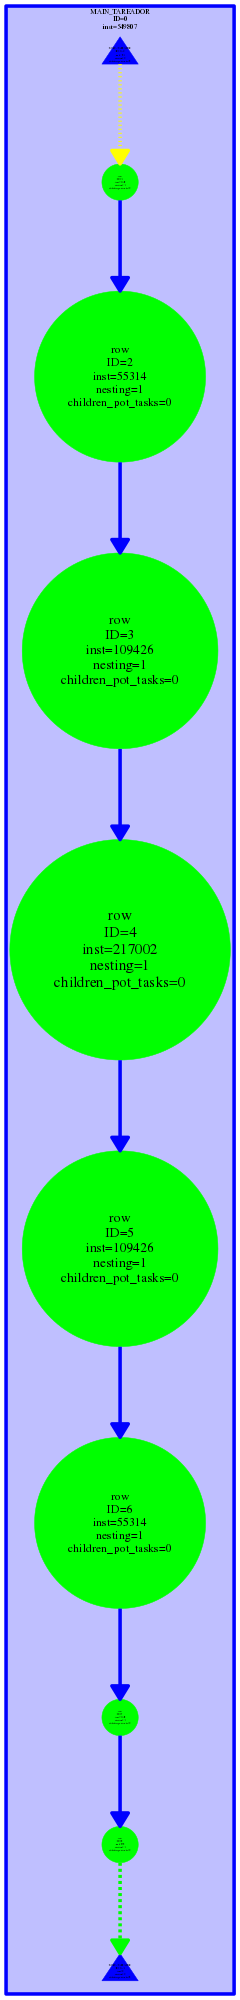
\includegraphics[scale=0.106]{./mandeld-tar_row}
	\caption{Mandeld-tar task decomposition graph using the row decomposition strategy.}
	\label{fig:mandeld-tar-row}
\end{figure}

In this strategy, the overhead time of creation and termination of tasks will be very small in comparison with the point strategy because it has to create less tasks. Nevertheless, it may happen that in a full row, all of its pixels must be white. In this case, it can happen that while other threads have finished their work, this other thread is still executing the row. Consequently, it is possible that the execution time may be bigger than in the point decomposition strategy.

\subsection{Characteristics of the TDG}

We saw in the previous sections that the execution of the mandel-tar has a very different task dependence graph than the execution of the mandeld-tar.

On the one hand, we can see that in mandel-tar every point is independent from the others. Consequently, we could parallelize that fragment of the code using OpenMP clauses.

On the other hand, in mandeld-tar we can see that all iterations have became sequential. In this situation, we do not gain anything by parallelizing the code, but we increase the execution time because of the overhead of creation and termination of tasks.

Using the \textit{Tareador} we could see which variable was responsible of creating those dependences. We did the following: Right Click into a task -$>$ Data View -$>$ Edges-out -$>$ Real Dependency. Figure \ref{fig:dependence_X11_COLOR_fake} shows the result we got.

\begin{figure}[H]
	\centering
	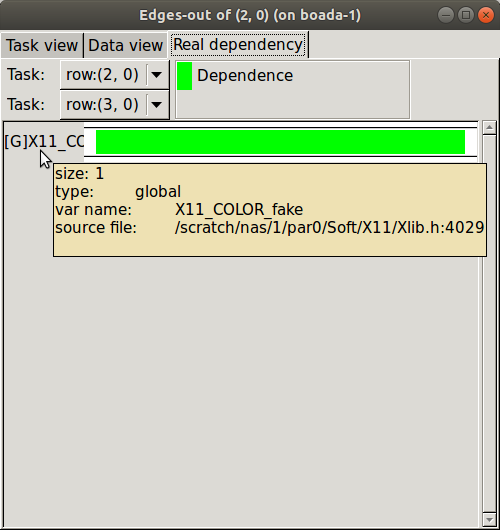
\includegraphics[scale=0.40]{./dependence_X11_COLOR_fake}
	\caption{Variable that provoques the dependences between tasks.}
	\label{fig:dependence_X11_COLOR_fake}
\end{figure}

We can see that there is only one variable that is causing all the dependences: X11\_COLOR\_fake. Observing the code, we noticed that the only difference between mandel-tar and mandeld-tar was a fragment of the code that was only executed in mode \_DISPLAY\_ (mandeld-tar):

\begin{figure}[H]
\begin{lstlisting}
#if _DISPLAY_
    /* Scale color and display point  */
    long color = (long) ((k-1) * scale_color) + min_color;
    if (setup_return == EXIT_SUCCESS) {
        XSetForeground (display, gc, color);
        XDrawPoint (display, win, gc, col, row);
    }
#else
    output[row][col]=k;
#endif
\end{lstlisting}
\caption{Fragment of the \textit{mandel-tar.c} code.}
\label{fig:display_code}
\end{figure}

Therefore, variable X11\_COLOR\_fake is used at least in one of the functions XSetForeground and XDrawPoint. We could protect this section of code in the parallel OpenMP code using the \textit{critical} clause to define a region of mutual exclusion where only one thread can be working at the same time.

\begin{figure}[H]
\begin{lstlisting}
#if _DISPLAY_
    /* Scale color and display point  */
    long color = (long) ((k-1) * scale_color) + min_color;
    
    #pragma omp critical
    if (setup_return == EXIT_SUCCESS) {
        XSetForeground (display, gc, color);
        XDrawPoint (display, win, gc, col, row);
    }
#else
    output[row][col]=k;
#endif
\end{lstlisting}
\caption{Fragment of the \textit{mandel-tar.c} code using the \textit{critical} clause to protect a fragment of the code.}
\label{fig:display_code}
\end{figure}



\textbf{\large\large{{FALTA AIXO:  Reason when each strategy/granularity should be used.}}}

\textbf{\large\large{{You also have to deliver the complete C source codes for Tareador instrumentation and all the
OpenMP parallelization strategies that you have done. Include both the PDF and source codes in
a single compressed tar file (GZ or ZIP). Only one file has to be submitted per group through the
Raco website.}}}

\section{Point decomposition in OpenMP}

In this section, we are going to explore different options in the OpenMP tasking model to express the Point decomposition for the Mandelbrot computation program. We will analyse the scalability and behaviour of these options.

%For the Point strategy implemented in OpenMP, describe and reason about how the performance has
%evolved for the three task versions of the code that you have evaluated, using the speed–up plots
%obtained and Paraver captures. 

%After that, explain the influence of the granularity control available in the taskloop construct, showing how the execution behaves when setting the number of tasks or
%iterations per task to 800, 400, 200, 100, 50, 25, 10, 5, 2 and 1, for example. Include the execution time
%and speed–up plots obtained in the strong scalability analysis (with -i 10000), again including Paraver
%captures to help you in the reasoning.

%\textbf{Optional}: taskgroup vs. taskwait: Include the parallel version that makes use of the taskgroup
%construct. Explain the two fundamental differences with taskwait and if they are relevant in this code.
%Also include the strong scalability analysis and use tracing to show the differences with taskwait.

\subsection{OpenMP Task Implementation}

The aim of this tasking model strategy is to create a task for each point. Figure \ref{code:task_implementation_point} show the OpenMP clauses we used to implement the task strategy (the code can be found in file \textit{mandel-omp-task-point.c} in codes folder).

\begin{figure}[H]
\begin{lstlisting}
for (int row = 0; row < height; ++row) {
	#pragma omp parallel
	#pragma omp single
    for (int col = 0; col < width; ++col) {
         #pragma omp task firstprivate(col)
         {
			...
			#pragma omp critical
	        if (setup_return == EXIT_SUCCESS) {
	        	XSetForeground (display, gc, color);
	        	XDrawPoint (display, win, gc, col, row);
	        }
			...
         }
     }
}
\end{lstlisting}
\caption{Fragment of the \textit{mandel-omp-task-point.c} code showing the OpenMP clauses to implement the task strategy.}
\label{code:task_implementation_point}
\end{figure}

Only one thread is creating all the tasks and inserting them into a pool of tasks, while the other threads are taking tasks from the pool and executing them. Thus, each iteration of the col loop will be executed as an independent task. The firstprivate clause is used in order to avoid problems of data races\footnote{We have not used the private clause because it initializes the variable with a random value, and we wanted the real value of the variable (iteration).}. Finally, the critical clause is used to honour the dependences we detected for the graphical version in the previous section. However, this section of the code will not be called since we will execute the code without the graphical version (only mandel-tar).

The following figure shows the execution flow of the program using the \textit{Paraver} tool.

\begin{figure}[H]
	\centering
	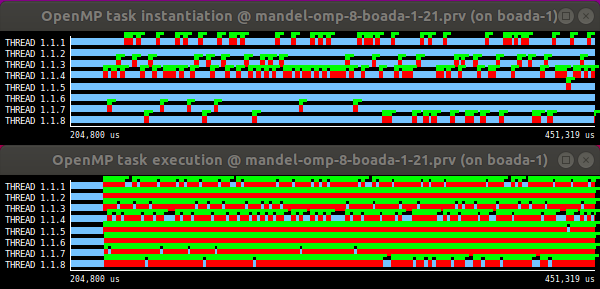
\includegraphics[scale=0.40]{./S2_OMP_tasks}
	\caption{Zoomed part of the execution flow using the task strategy.}
	\label{fig:dependence_X11_COLOR_fake}
\end{figure}

We can observe the effect of the single clause. In the upper part (task instantiation) only one thread is creating the tasks and inserting them in the task pool. In the bottom part (task execution) we can see that the other threads execute the tasks as they are put in the pool. The role of the task creator changes every time we finish a row.

In total, there are 640000 tasks created and executed. This is because the image has size $800 \times 800$. We have seen this using the "OMP\_parallel\_functions.cfg" i "OMP\_state\_profile.cfg" configurations. Figure XXXXXXXXXXXXXXXX shows the results obtained.

The parallel construct is executed 1 time and the single worksharing construct is executed 1 time for each thread. All threads will execute the single lines but only one will "gain". This thread will be responsible for creating the tasks of that row.

Finally, figures \ref{fig:mandel-omp-10000-strong-21-time} and \ref{fig:mandel-omp-10000-strong-21-speedup} show the time and speedup plots.

\begin{figure}[H]
\centering
\begin{minipage}[b]{0.4\linewidth}
  \centering
  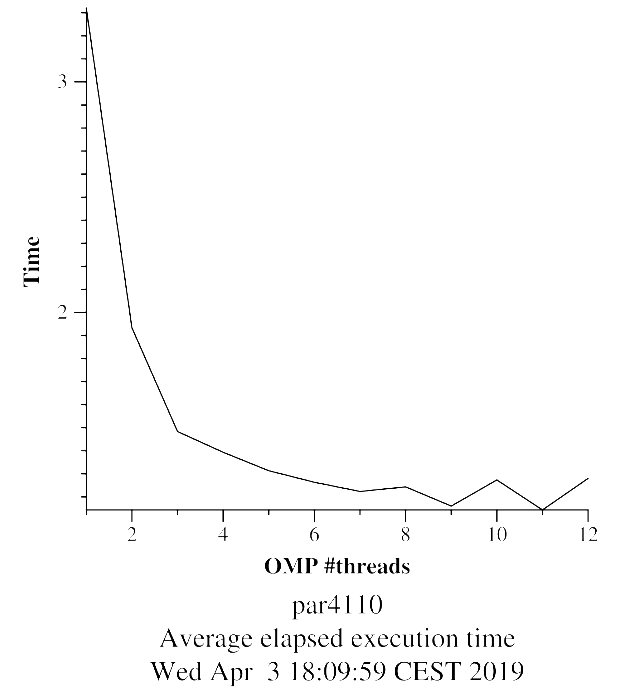
\includegraphics[scale=0.5]{./mandel-omp-10000-strong-21-time}
  \caption{Execution time plot varying the number of threads.}
  \label{fig:mandel-omp-10000-strong-21-time}
\end{minipage}%
\hspace{0.5cm}
\begin{minipage}[b]{0.4\linewidth}
  \centering
  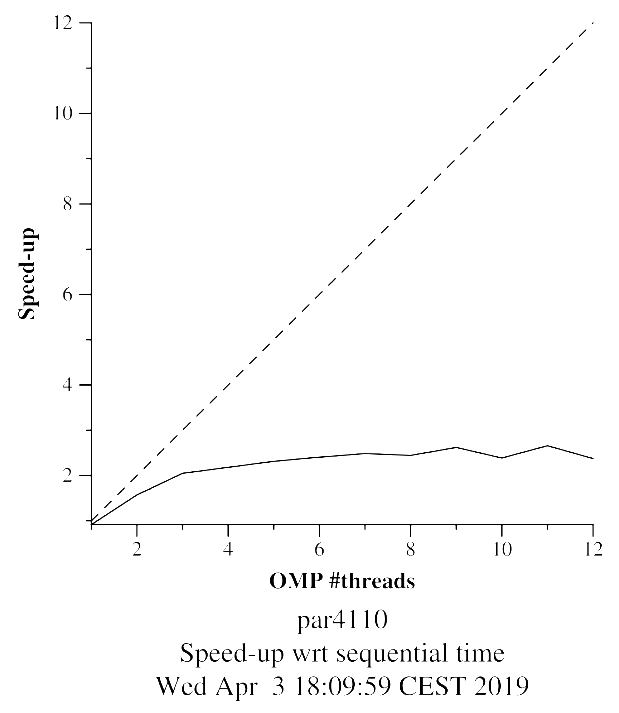
\includegraphics[scale=0.5]{./mandel-omp-10000-strong-21-speedup}
  \caption{Speedup plot varying the number of threads.}
  \label{fig:mandel-omp-10000-strong-21-speedup}
\end{minipage}
\end{figure}

In the first plot, the execution time is reduces as we increase the number of threads until the time stays constant. However, we think that if we increase a lot the number of threads, the execution time would end up increasing because of the overheads.

On the other hand, in the second plot the speedup increases a lot with 2-4 threads but ends up constant as we increase the number of threads.

\textbf{\large{\large{REPASSAR EL SEGUENT: The scalability is not appropiate because the speedup stays at 2 (reduction of time of T$_1$) even though we have 8 threads.}}}

\subsubsection{OpenMP Taskwait Variant}

In this variant of the previous code, only one thread (the one that gets access to the single region), traverses all iterations of the row and col loops, generating a task for each iteration of the innermost loop (point). To do it, we have introduced "\#pragma omp taskwait" at the end of each iteration of a row. Consequently, the creator thread must wait until all tasks for a row finish. After that, the thread will advace one iteration of the row loop and generate a new bunch of tasks. This new version of the code can be found in \textit{mandel-omp-task-point-taskwait.c}.

\begin{figure}[H]
\begin{lstlisting}
#pragma omp parallel
#pragma omp single
for (int row = 0; row < height; ++row) {
	for (int col = 0; col < width; ++col) {
		#pragma omp task firstprivate(row, col)
		{
			...
		}
	}
	#pragma omp taskwait // waiting point for all child tasks
}
\end{lstlisting}
\caption{Fragment of the \textit{mandel-omp-task-point-taskwait.c} code showing the OpenMP clauses to implement the task strategy with the taskwait variant.}
\label{code:task_implementation_point_taskwait}
\end{figure}

The number of created and executed tasks is still 640000 as we have not modified the size of the image. Nevertheless, even though the number of calls to parallel is the same, the number of calls to the single worksharing construct will only be 8, the number of threads. Besides, the taskwait clause will be executed 800 times (number of rows). The granularity is the same than before. Each task has exactly one iteration of the for.

Figures \ref{fig:mandel-omp-10000-strong-22-time} and \ref{fig:mandel-omp-10000-strong-22-speedup} show again the time and speedup plots. We have not noticed any significant difference between these plots and the plots of the previous section.

\begin{figure}[H]
\centering
\begin{minipage}[b]{0.4\linewidth}
  \centering
  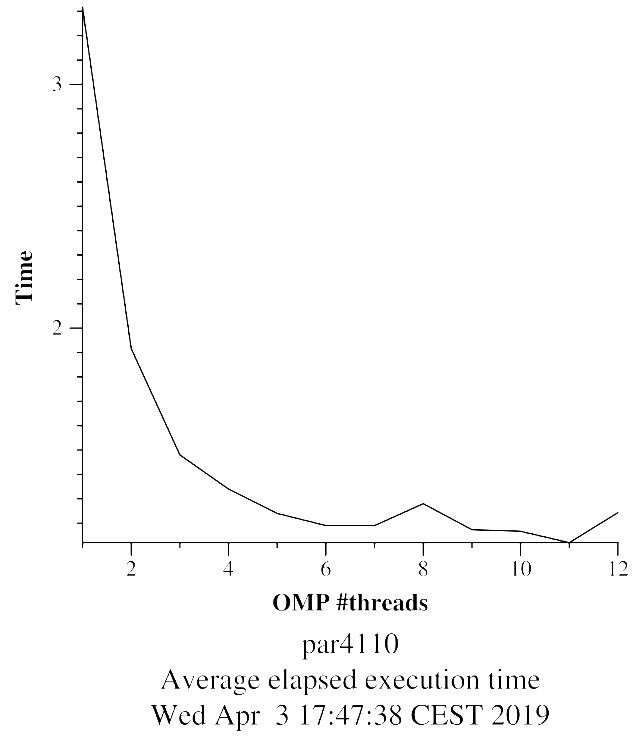
\includegraphics[scale=0.5]{./mandel-omp-10000-strong-22-time}
  \caption{Execution time plot varying the number of threads.}
  \label{fig:mandel-omp-10000-strong-22-time}
\end{minipage}%
\hspace{0.5cm}
\begin{minipage}[b]{0.4\linewidth}
  \centering
  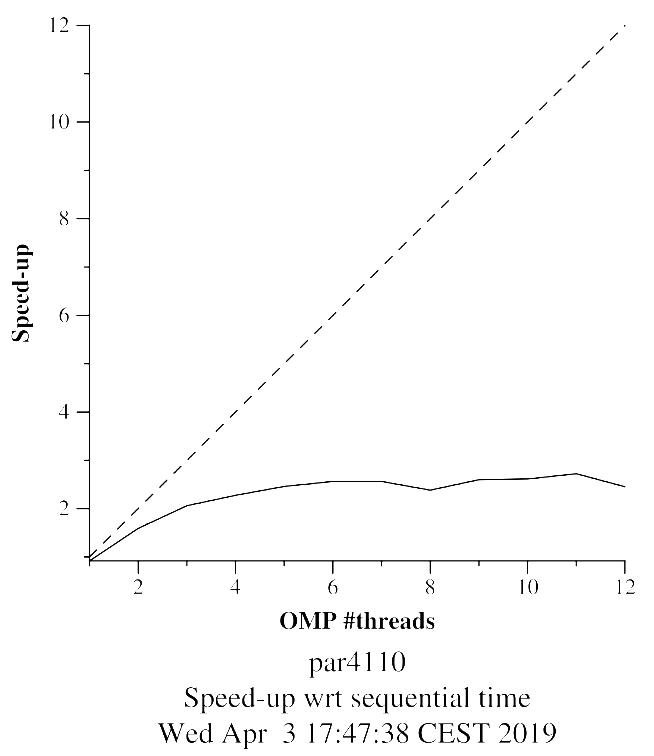
\includegraphics[scale=0.5]{./mandel-omp-10000-strong-22-speedup}
  \caption{Speedup plot varying the number of threads.}
  \label{fig:mandel-omp-10000-strong-22-speedup}
\end{minipage}
\end{figure}

\subsubsection{OpenMP Taskgroup Variant}

In this other variant, we define a region in the program where the thread will wait for the termination of all descendant (not only child) tasks. Figure \ref{code:task_implementation_point_taskgroup} shows a section of the modified code that can be found in file \textit{mandel-omp-task-point-taskgroup.c} inside the codes directory. Now, the pixels are generated without any specific order.

\begin{figure}[H]
\begin{lstlisting}
#pragma omp parallel
#pragma omp single
for (int row = 0; row < height; ++row) {
	#pragma omp taskgroup
	{
		for (int col = 0; col < width; ++col) {
        	#pragma omp task firstprivate(row, col)
        	{
        		...
			}
		}
	}
}
\end{lstlisting}
\caption{Fragment of the \textit{mandel-omp-task-point-taskgroup.c} code showing the OpenMP clauses to implement the task strategy with the taskgroup variant.}
\label{code:task_implementation_point_taskgroup}
\end{figure}

Figures \ref{fig:mandel-omp-10000-strong-23-time} and \ref{fig:mandel-omp-10000-strong-23-speedup} show again the time and speedup plots. We have not noticed any significant difference between these plots and the plots of the two previous sections.

\begin{figure}[H]
\centering
\begin{minipage}[b]{0.4\linewidth}
  \centering
  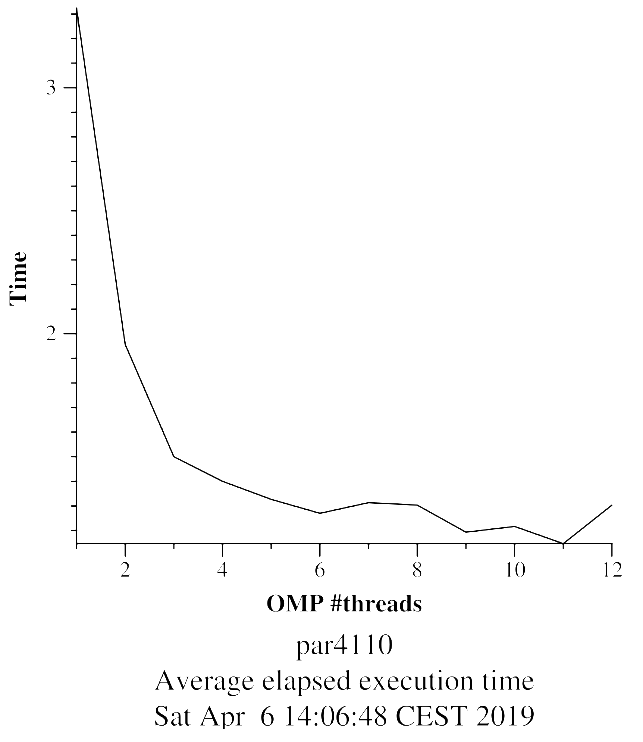
\includegraphics[scale=0.5]{./mandel-omp-10000-strong-23-time}
  \caption{Execution time plot varying the number of threads.}
  \label{fig:mandel-omp-10000-strong-23-time}
\end{minipage}%
\hspace{0.5cm}
\begin{minipage}[b]{0.4\linewidth}
  \centering
  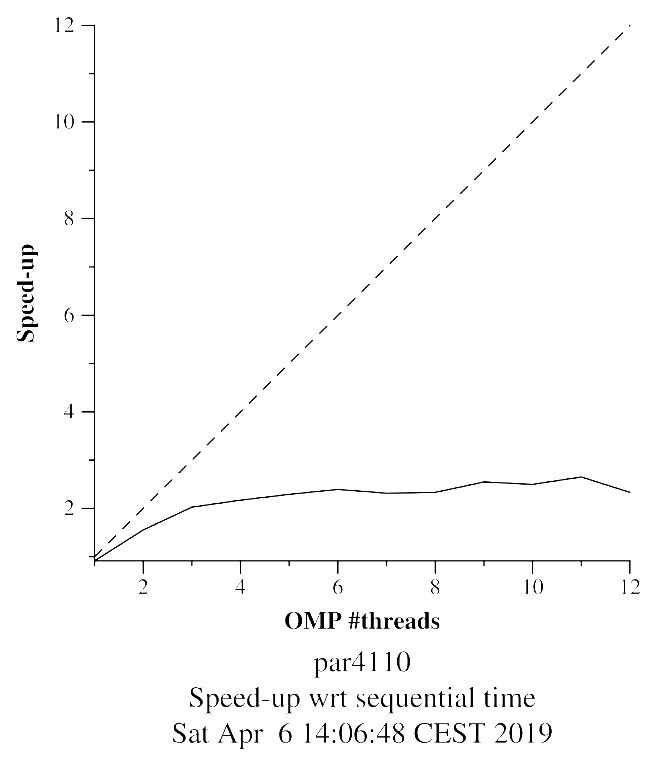
\includegraphics[scale=0.5]{./mandel-omp-10000-strong-23-speedup}
  \caption{Speedup plot varying the number of threads.}
  \label{fig:mandel-omp-10000-strong-23-speedup}
\end{minipage}
\end{figure}

\textbf{\large{\large{FALTA: Do you think the taskwait construct in Figure 2.2 is really necessary? Or in other words, is it
necessary to wait for the termination of all tasks in a row before generating the tasks for the next rows?
Modify the code in mandel-omp.c to remove this task barrier and repeat the previous evaluation (scalability and tracing). Has the number of tasks created/executed changed? Why the threads generating
tasks stops task generation, then executes some tasks, and then proceeds generating new tasks?}}}

El taskwait no es necessari ja que les taskes no tenen res a veure unes amb les altres a la hora de calcular. Per tant tan es l'ordre de generacio de les tasques, entre diferents rows. Em observat que ens dona els mateixos resultats amb l'execució anterior. El nombre de taskes creades i executades no varien respecte l'execució anterior. Això es culpa de que la bossa de taskes que té l'omp és limitada, per això arriba un punt que de forma intel·ligent el thread 0 atura la creació de taskes, per executar-ne i així poder disminuir la quantitat total de taskes a la bossa.

\end{document}
